\section{Zustandsbasierte Systeme}

\subsection{Asynchrone vs. synchrone FSM}

\begin{minipage}[t]{0.48\columnwidth}
    \raggedright
    \begin{outline}
        \1 \textbf{Asynchron}
            \2 geänderte Inputsignale führen \textbf{direkt} zur Zustandsänderung
            \2 schneller, aber enorm anfällig auf Glitches
    \end{outline}
\end{minipage}
\hfill
\begin{minipage}[t]{0.48\columnwidth}
    \raggedright
    \begin{outline}
        \1 \textbf{Synchron}
            \2 Inputsignale werden nur zu diskreten Zeitpunkten betrachtet \\
                \textrightarrow\ getaktete Systeme
    \end{outline}
\end{minipage}

\vspace{0.2cm}
%TODO: check if this is finished
\begin{outline}
    \1 Softwareimplementationen sind eigentlich immer \textbf{synchron}, da Rechner getaktet sind
    \1 Rein softwareseitig besteht die Problematik der Asynchronizität nicht
\end{outline}


\subsection{Finite State Machines (FSM)}


\subsubsection{Mealy-Automat}

\subsubsection{Moore-Automat}
% Bondi: alles als Moore modellieren

\subsubsection{Medvedjev}
%hier nicht weiter behandelt...?
% Zustand = Output


\subsection{State-Event-Diagramm (Zustandsdiagramm)}

% Beschreibung


\example{State-Event-Diagramm -- Moore Automat}

% \begin{center}
%     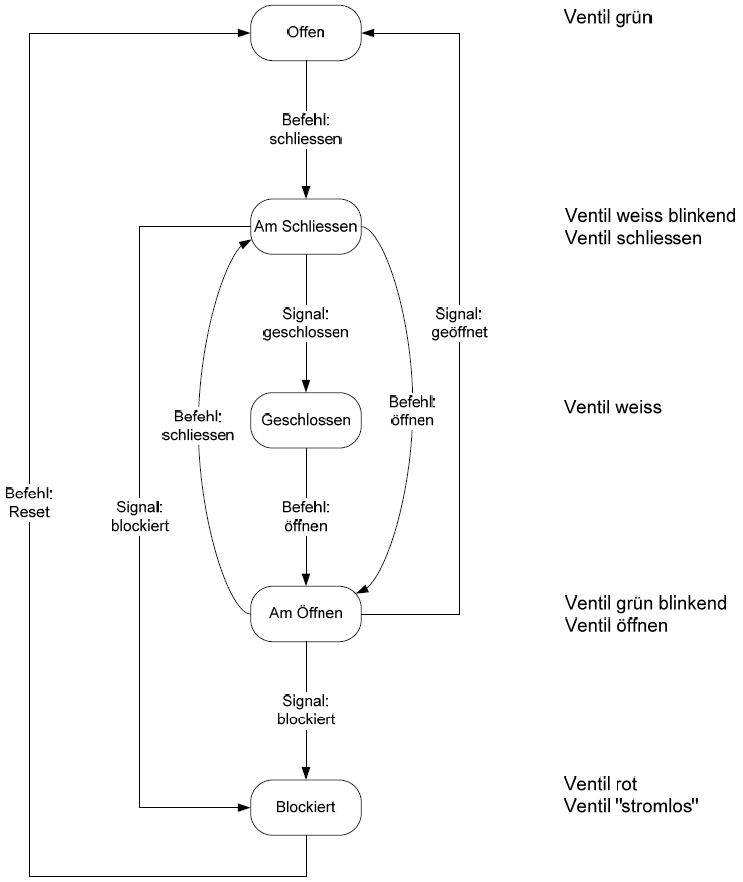
\includegraphics[width=0.8\columnwidth]{images/state_event_example.png}
% \end{center}

